\documentclass{article}
\usepackage{amsmath}
\usepackage{mathtools}
\usepackage{gensymb}
\usepackage[a4paper,inner=1.5cm,outer=1.5cm,top=2cm,bottom=0.5cm]{geometry} 
\usepackage{xcolor}                    
\usepackage{tikz}                           
\usepackage{multicol}
\usepackage{pgfplots}
\usetikzlibrary{calc}
\usetikzlibrary{intersections}
\usetikzlibrary{intersections,calc,angles,quotes}
\usetikzlibrary{shapes,arrows,positioning,decorations.pathreplacing,calc}
\usetikzlibrary{calc,angles,positioning,intersections,quotes,decorations.markings}
\usepackage{tkz-euclide}
\usetikzlibrary{backgrounds}
\usetikzlibrary{calc,through}
\usetikzlibrary{angles}
\usetikzlibrary{fadings}
\usetikzlibrary{shapes.geometric}
\usetikzlibrary{shapes.symbols}
\usepackage{draftwatermark}
\usepackage{mathptmx}

\SetWatermarkText{\textcolor{black!30}{Mathema Shukur}}
\SetWatermarkFontSize{2 cm}
\usepackage[utf8]{inputenc}
\usepackage{fontspec}

\setmainfont{[Kalpurush.ttf]}
\newfontface{\en}{[Arial.ttf]} %%this is optional, if you want to use a secondary font. Any english font is supported
\newlength\Radius
\setlength\Radius{4cm}
\begin{document} 
	\Large
	\textcolor{red}{Welcome To} 
	\\
	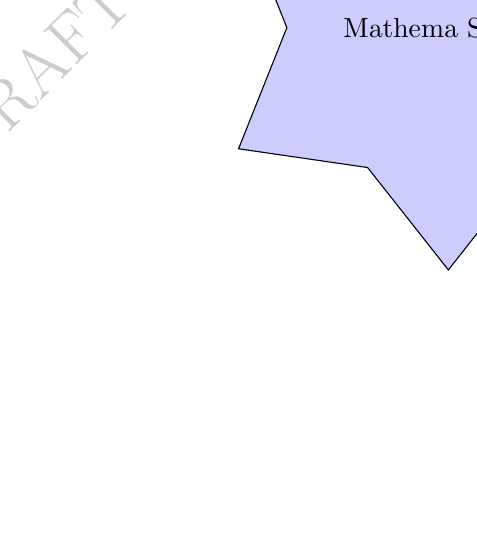
\begin{tikzpicture}
		\tikz \node [fill=blue!20,star,star points=6,draw] {Mathema Shukur };
	\end{tikzpicture}
	\\
	যাদের জন্যে প্রযোজ্যঃ  	\textcolor{magenta}{একাদশ ও দ্বাদশ শ্রেণীর শিক্ষার্থী} \\
	বিষয়ঃ \textcolor{magenta}{উচ্চতর গণিত ১ম পত্র} \\
	অধ্যায়ঃ \textcolor{magenta}{৩-সরলরেখা}\\ 
	Subtopicঃ  \textcolor{magenta}{  সরলরেখার বিভিন্ন আকারের সমীকরণ নির্ণয় করা   }\\
	\\
	\textcolor{blue}{(1)	ঢাল বিন্দু আকার Point slope form}\\
	\\
	$(y-y_1)=m(x-x_1)$\\
	\\
	\textcolor{red} {(2)  দুই বিন্দু আকার 	Two point form}\\
	\\
	$y-y_1=\left(\frac{y_1-y_2}{x_1-x_2}\right)(x-x_1)$\\
	\\
	\textcolor{green}{ (3) ঢাল খণ্ডন আকার 	Slope intercept form}\\
	\\
	$y=mx+c$\\
	\\
	\textcolor{cyan}{ (4) দ্বি খণ্ডন আকার  Two	Intercept form}\\
	\\
	$\frac{x}{a}+\frac{y}{b}=1$\\
	\\
	\vspace{6cm}
	\\
	\textcolor{cyan}{ (4) দ্বি খণ্ডন আকার  Two	Intercept form}\\
\\
$\frac{x}{a}+\frac{y}{b}=1$\\
	\\
	$x-$ অক্ষের খণ্ডিত অংশ $a$,\qquad $y-$ অক্ষের খণ্ডিত অংশ $b$\\
	\\ 
	সরলরেখাটি $x-$ অক্ষকে $(a,0)$ বিন্দুতে  ছেদ করে\\
	\\
		সরলরেখাটি $y-$ অক্ষকে $(0,b)$ বিন্দুতে ছেদ করে\\
		\\ 
	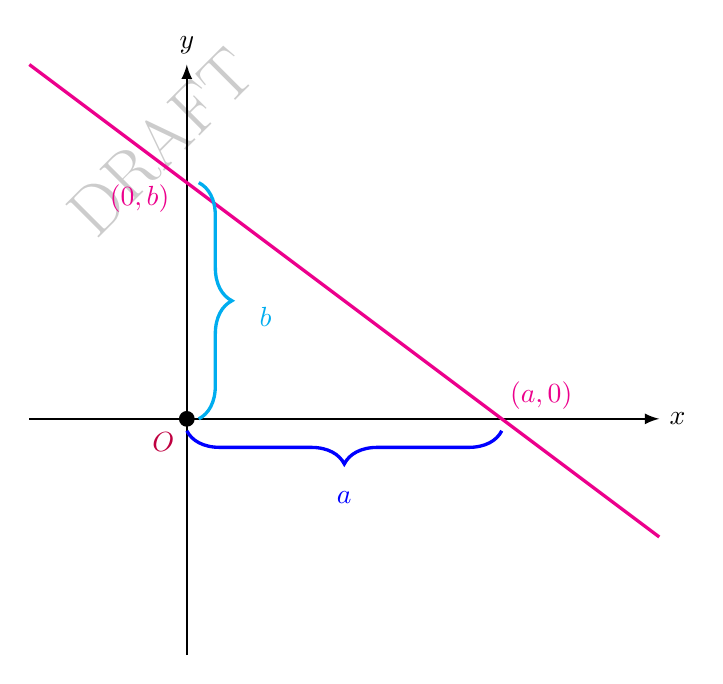
\begin{tikzpicture}[transform shape,scale=1]
		\draw [-latex,thick](-2,0) -- (6,0) node[right] {$x$} coordinate(x axis);
		\draw [-latex,thick](0,-3) -- (0,4.5) node[above] {$y$} coordinate(y axis);
		\fill[black] (0,0) circle (1 mm);
		\node at (-0.3,-0.3) {$\textcolor{purple}{O}$};	
		\node at (1,1.3) {$\textcolor{cyan}{b}$};	
			\node at (2,-1) {$\textcolor{blue}{a}$};	
				\node at (4.5,0.3) {$\textcolor{magenta}{(a,0)}$};
					\node at (-0.6,2.8) {$\textcolor{magenta}{(0,b)}$};
		\draw[very thick,magenta] (-2,4.5)--(6,-1.5);	
		\draw [cyan,very thick,decorate,decoration={brace,amplitude=12pt,mirror,raise=1ex}]
		(0,0) -- (0,3);
			\draw [blue,very thick,decorate,decoration={brace,amplitude=12pt,mirror,raise=1ex}]
		(0,0) -- (4,0);
	\end{tikzpicture}
\\ 
	সিলেট বোর্ড-২০২১\\ 
	$3x-4y+12=0$ সরলরেখা দ্বারা $x-$ অক্ষের খণ্ডিত অংশের ও $y-$ অক্ষের খণ্ডিত অংশের দৈর্ঘ্য নির্ণয় কর \\ 
	\\ 
	\begin{align*}
	3x-4y+12&=0\\
	\\
		3x-4y&=-12\\
		\\
		\frac{3x}{-12}+\frac{-4y}{-12}=\frac{-12}{-12}\\
		\\
		\frac{x}{-4}+\frac{y}{3}&=1\\
		&\boxed{\textcolor{blue}{\frac{x}{a}+\frac{y}{b}=1}}\\
	\end{align*}
\\
$x-$ অক্ষের খণ্ডিত অংশের  দৈর্ঘ্য $a=|-4|=4$ ও $y-$ অক্ষের খণ্ডিত অংশের দৈর্ঘ্য $b=3$\\
\\ 
		\begin{tikzpicture}[transform shape,scale=1]
		\draw [-latex,thick](-8,0) -- (4,0) node[right] {$x$} coordinate(x axis);
		\draw [-latex,thick](0,-3) -- (0,6) node[above] {$y$} coordinate(y axis);
		\fill[black] (0,0) circle (1 mm);
		\node at (-0.3,-0.3) {$\textcolor{purple}{O}$};	
		
		\draw[very thick,magenta] (-8,-3)--(4,6);	
		\node at (0.8,3) {$\textcolor{magenta}{\left(0,3\right)}$};
		\node at (-3.7,-0.5) {$\textcolor{magenta}{\left(-4,0\right)}$};
	\end{tikzpicture}
	\\
		যশোর বোর্ড-২০২১\\
	$\frac{x}{5}+\frac{y}{6}=1$ রেখাটি অক্ষদ্বয়ের সাথে যে ত্রিভুজ গঠন করে তার ক্ষেত্রফল নির্ণয় কর \\ 
	\\ 
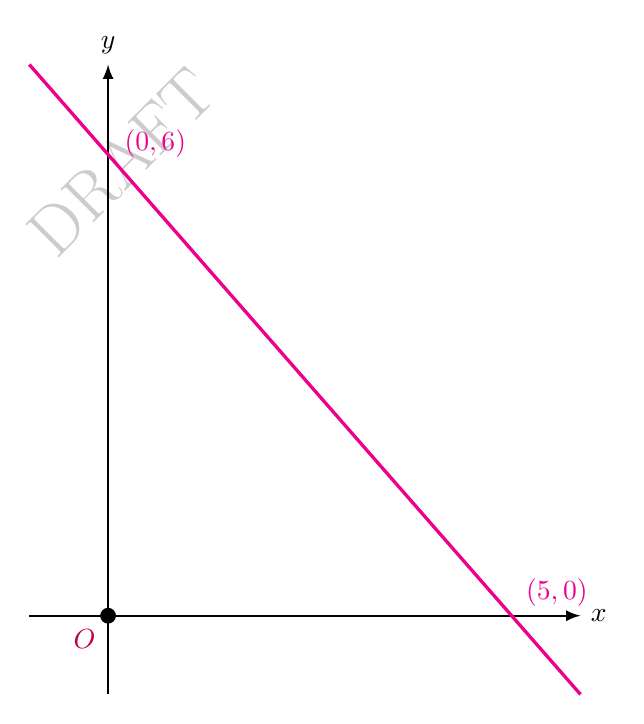
\begin{tikzpicture}[transform shape,scale=1]
	\draw [-latex,thick](-1,0) -- (6,0) node[right] {$x$} coordinate(x axis);
	\draw [-latex,thick](0,-1) -- (0,7) node[above] {$y$} coordinate(y axis);
	\fill[black] (0,0) circle (1 mm);
	\node at (-0.3,-0.3) {$\textcolor{purple}{O}$};	
	
	\draw[very thick,magenta] (6,-1)--(-1,7);	
	\node at (5.7,0.3) {$\textcolor{magenta}{\left(5,0\right)}$};
	\node at (0.6,6) {$\textcolor{magenta}{\left(0,6\right)}$};
\end{tikzpicture}
\\
ত্রিভুজের ভূমি=  $x-$ অক্ষের খণ্ডিত অংশের  দৈর্ঘ্য $=5$\\
\\
ত্রিভুজের উচ্চতা =$y-$ অক্ষের খণ্ডিত অংশের দৈর্ঘ্য $=6$ \\
\\ 
ত্রিভুজের ক্ষেত্রফল $=\frac{1}{2}\times 5\times 6=15$\\
\\ 
	দিনাজপুর বোর্ড-২০২১\\
 $3y-2x+6=0$ রেখাটি অক্ষদ্বয়ের সাথে যে ত্রিভুজ গঠন করে তার ক্ষেত্রফল নির্ণয় কর \\ 
	\\
	\\
	\\
		সিলেট বোর্ড-২০২১\\ 
	অক্ষ দুইটি দ্বারা $5x-10y=7$ সরলরেখার খণ্ডিত অংশের মধ্য বিন্দুর স্থানাঙ্ক নির্ণয় কর \\ 
	\\ 
	\begin{align*}
	5x-10y&=7\\
	\\
	\frac{5x}{7}+\frac{-10y}{7}&=\frac{7}{7}\\
	\\
	\frac{x}{\frac{7}{5}}+\frac{y}{-\frac{7}{10}}&=1
	\end{align*}
\\
	সরলরেখাটি $x-$ অক্ষকে $A\left(\frac{7}{5},0\right)$ বিন্দুতে  ছেদ করে\\
\\
সরলরেখাটি $y-$ অক্ষকে $B\left(0,-\frac{7}{10}\right)$ বিন্দুতে ছেদ করে\\
\\ 
খণ্ডিত অংশ $AB$ এর মধ্যবিন্দুর স্থানাঙ্ক $\left(\frac{\frac{7}{5}+0}{2},\frac{0-\frac{7}{10}}{2}\right)=\left(\frac{7}{10},\frac{-7}{20}\right)$\\
\\
		\begin{tikzpicture}[transform shape,scale=1]
		\draw [-latex,thick](-3,0) -- (11,0) node[right] {$x$} coordinate(x axis);
		\draw [-latex,thick](0,-5) -- (0,2) node[above] {$y$} coordinate(y axis);
		\fill[black] (0,0) circle (1 mm);
			\fill[blue] (3.5,-1.75) circle (1 mm);
				\node at (4.5,-2) {$\textcolor{blue}{\left(\frac{7}{10},\frac{-7}{20}\right)}$};
		\node at (-0.3,-0.3) {$\textcolor{purple}{O}$};	

		\draw[very thick,magenta] (11,2)--(-3,-5);	
	\node at (6.5,0.5) {$\textcolor{magenta}{A\left(\frac{7}{5},0\right)}$};
\node at (1.5,-3.5) {$\textcolor{magenta}{B\left(0,-\frac{7}{10}\right)}$};
	\end{tikzpicture}
\end{document}